\documentclass[a4paper,12pt]{article}

\usepackage[utf8]{inputenc}
\usepackage[italian]{babel}
\usepackage{amsmath}
\usepackage{geometry}
\usepackage{listings}
\usepackage{hyperref}
\usepackage{graphicx}
\usepackage{booktabs}
\usepackage{caption}
\usepackage{subcaption}
\usepackage{float}

\geometry{margin=2.5cm}

\graphicspath{{Progettazione/cpi/}{Progettazione/heat/}{Progettazione/factorize/}}

\lstset{
    basicstyle=\ttfamily\small,
    breaklines=true,
    frame=single,
    numbers=left,
    numberstyle=\tiny,
    xleftmargin=1.5em,
    language=C
}

\title{Relazione Laboratorio HPC -- Esercitazione 3\\
\large Progettazione di programmi paralleli}
\author{Federico Becchi}
\date{Giugno 2026}

\begin{document}

\maketitle

% =========================================================
\section{Introduzione}

In questa esercitazione vengono analizzati tre programmi seriali in C --- \texttt{cpi}, \texttt{heat} e \texttt{factorize} --- dal punto di vista della progettazione della parallelizzazione. Per ciascuno si analizzano: la legge di Amdahl, il partizionamento del carico, la decomposizione del dominio (metodo, granularit\`a), l'impatto sulla comunicazione, il bilanciamento del carico e la gestione dei thread/processi.

I test sono stati eseguiti su:
\begin{itemize}
    \item \textbf{PC locale}: MacBook Air con chip Apple M3, macOS, architettura ARM64
    \item \textbf{Cluster HPC Ateneo}: nodo \texttt{ui01.hpc.unipr.it}, Intel Xeon Gold 6238R @ 2.20 GHz, architettura x86\_64, gestito tramite SLURM
\end{itemize}

% =========================================================
\section{Esercizio CPI -- Calcolo di Pi greco}

\subsection{Descrizione dell'algoritmo}

Il programma \texttt{cpi.c} calcola $\pi$ tramite integrazione numerica con il metodo dei rettangoli nell'intervallo $[0,1]$. Sono disponibili due funzioni:
\begin{itemize}
    \item \texttt{f1(n)}: calcola $\displaystyle\sum_{i=1}^{n} \sqrt{1-x_i^2}$, dove l'integrale corrisponde all'area di un quarto di cerchio ($\pi/4$)
    \item \texttt{f2(n)}: calcola $\displaystyle\sum_{i=1}^{n} \frac{1}{1+x_i^2}$, dove l'integrale vale $\arctan(1) = \pi/4$
\end{itemize}
con $x_i = h \cdot (i - 0.5)$ e $h = 1/n$. Il risultato finale \`e $\pi = 4 \cdot h \cdot \text{sum}$.

Il programma misura separatamente il tempo non parallelizzabile $t_{np}$ (gestione input, inizializzazione) e il tempo parallelizzabile $t_p$ (ciclo \texttt{for} di integrazione) tramite \texttt{clock\_gettime()}.

\subsection{Struttura del codice}

\begin{itemize}
    \item \texttt{options()}: gestione parametri da CLI (\texttt{-n} per il numero di intervalli)
    \item \texttt{f1()}, \texttt{f2()}: le due funzioni di integrazione
    \item Il ciclo \texttt{for} principale: tutte le iterazioni sono \textbf{indipendenti} tra loro
\end{itemize}

\subsection{Legge di Amdahl}

Il programma \texttt{cpi+amdahl.c} aggiunge una chiamata \texttt{usleep(s)} per simulare una parte di codice non parallelizzabile, parametrizzabile con l'opzione \texttt{-s}. Lo speedup teorico secondo Amdahl \`e:
\[
S(P) = \frac{t_{np} + t_p}{t_{np} + t_p / P}
\]

Dall'esecuzione sul PC con $n = 10^8$ e \texttt{usleep(100000)} si ottengono $t_p = 0.10083$~s e $t_{np} = 0.15294$~s, con una frazione parallelizzabile del 39\%. La Figura~\ref{fig:amdahl_pc} mostra come lo speedup satura rapidamente: con 32 processori si otterrebbe uno speedup massimo di circa $1/0.61 \approx 1.64$.

Sul cluster (Figura~\ref{fig:amdahl_cluster}) la percentuale parallelizzabile scende al 15\%, portando a uno speedup massimo teorico di circa $1/0.85 \approx 1.18$. Questo dimostra che la parte seriale domina e limita fortemente lo scaling.

\begin{figure}[H]
\centering
\begin{subfigure}{0.48\textwidth}
    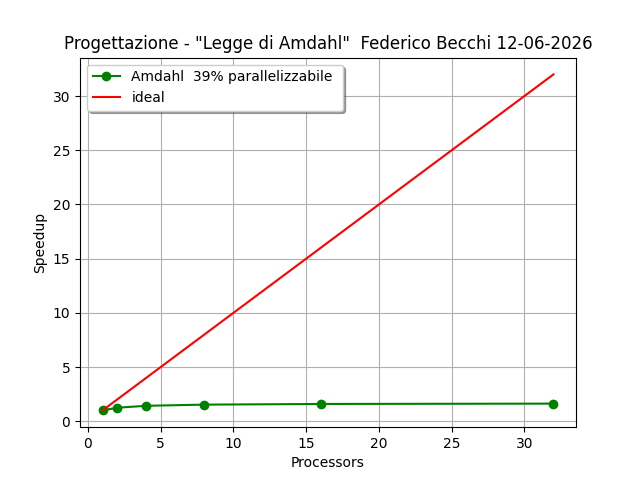
\includegraphics[width=\textwidth]{cpi+amdahl.png}
    \caption{PC locale -- 39\% parallelizzabile}
    \label{fig:amdahl_pc}
\end{subfigure}
\hfill
\begin{subfigure}{0.48\textwidth}
    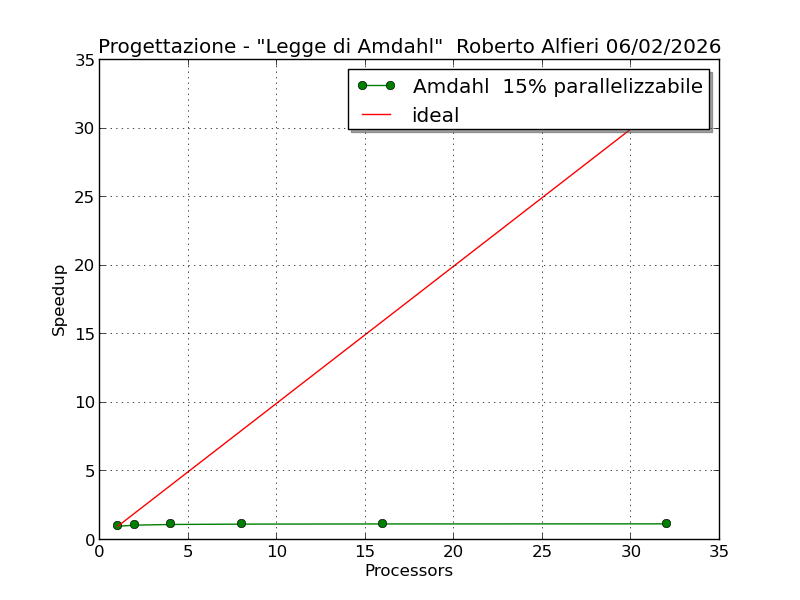
\includegraphics[width=\textwidth]{cpi+amdahl_cluster.png}
    \caption{Cluster -- 15\% parallelizzabile}
    \label{fig:amdahl_cluster}
\end{subfigure}
\caption{Legge di Amdahl per il programma CPI con \texttt{usleep} simulato.}
\label{fig:amdahl}
\end{figure}

Senza la \texttt{usleep} (programma \texttt{cpi.c} puro), la parte non parallelizzabile \`e trascurabile e ci si aspetta uno speedup quasi lineare.

\subsection{Decomposizione del dominio}

La parte parallelizzabile \`e il ciclo \texttt{for} che calcola la somma delle aree dei rettangoli. La decomposizione \`e \textbf{1D} lungo l'indice $i$:

\begin{itemize}
    \item \textbf{Grana grossa}: gli $n$ intervalli vengono divisi in $P$ parti contigue di dimensione $n/P$. Ogni processore calcola la somma parziale del proprio blocco.
    \item \textbf{Grana fine}: gli intervalli vengono divisi in piccoli chunk distribuiti a rotazione (\textit{round-robin}) o su richiesta (\textit{dynamic scheduling}).
\end{itemize}

Entrambe le strategie funzionano bene perch\'e il carico computazionale per iterazione \`e uniforme (stessa operazione per ogni $x_i$), quindi il bilanciamento \`e naturalmente ottimale.

\subsection{Overhead di comunicazione}

Al termine del calcolo, ogni processo invia la propria somma parziale al processo principale per un'operazione di \textbf{riduzione} (somma). Vengono scambiati $P-1$ messaggi di 8 byte (un \texttt{double}). L'overhead di comunicazione \`e trascurabile.

\subsection{Sincronizzazione}

\`E necessaria una barriera implicita prima della riduzione per attendere che tutti i processi abbiano completato il calcolo. Con grana fine e scheduling dinamico non ci sono tempi di idle; con grana grossa, basta che i sottodomini siano di pari dimensione.

Lo startup (creazione di $P$ processi/thread) avviene una sola volta ed \`e trascurabile.

\textbf{Conclusione}: tutti gli overhead sono trascurabili per CPI. Ci si aspetta uno scaling ottimale dello speedup.

% =========================================================
\section{Esercizio Heat -- Propagazione del calore}

\subsection{Descrizione dell'algoritmo}

Il programma \texttt{heat.c} simula la propagazione del calore su una superficie rettangolare $NX \times NY$ (default $512 \times 512$) utilizzando il metodo iterativo di \textbf{Jacobi}. Ad ogni iterazione, la temperatura di ogni cella interna viene aggiornata come media dei 4 vicini (N, S, E, W):
\[
T_{new}[i,j] = \frac{1}{4}\left(T[i+1,j] + T[i-1,j] + T[i,j+1] + T[i,j-1]\right)
\]

\subsection{Struttura del codice}

Il ciclo principale esegue \texttt{MAX\_ITER} iterazioni (default 1000):
\begin{enumerate}
    \item \textbf{Swap} dei puntatori \texttt{h\_T\_old} $\leftrightarrow$ \texttt{h\_T\_new} (evita copie di memoria)
    \item \textbf{Inizializzazione sorgenti}: \texttt{Init\_center()} (rettangolo centrale a 1.0), \texttt{Init\_left()} (bordo sinistro a 1.0), \texttt{Init\_top()} (bordo superiore a 1.0)
    \item \textbf{Condizioni periodiche}: \texttt{copy\_rows()} e \texttt{copy\_cols()} copiano i bordi per realizzare condizioni al contorno periodiche (la superficie \`e topologicamente un toro)
    \item \textbf{Jacobi}: aggiornamento di tutte le celle interne
\end{enumerate}

Il ciclo esterno temporale \textbf{non pu\`o essere parallelizzato} poich\'e rappresenta la progressione temporale: ogni iterazione dipende dai risultati della precedente.

\subsection{Legge di Amdahl}

La parte parallelizzabile \`e la funzione \texttt{Jacobi\_Iterator\_CPU()}, che domina il tempo di esecuzione. La parte non parallelizzabile comprende l'inizializzazione delle sorgenti (\texttt{Init\_center}, \texttt{Init\_left}, \texttt{Init\_top}) e le copie per le condizioni periodiche. Per griglie grandi, la funzione Jacobi \`e la componente dominante e la frazione seriale diventa piccola.

\subsection{Decomposizione del dominio}

La funzione Jacobi pu\`o essere parallelizzata distribuendo le righe della superficie tra i processi/thread. Si utilizza una \textbf{decomposizione 1D per righe}:

\begin{itemize}
    \item \textbf{Grana grossa} (memoria distribuita -- MPI): la griglia viene divisa in $P$ bande orizzontali di $NY/P$ righe ciascuna. Ogni processo lavora sul proprio sottodominio.
    \item \textbf{Grana fine} (memoria condivisa -- OpenMP): ogni iterazione del loop esterno (su $j$) pu\`o essere assegnata a un thread diverso. Con \texttt{\#pragma omp parallel for collapse(2)} si pu\`o parallelizzare anche sul doppio indice.
\end{itemize}

\subsection{Comunicazione -- Ghost cells}

Nel modello a \textbf{memoria distribuita}, per calcolare la nuova temperatura di una riga al bordo del sottodominio, occorre accedere alla riga adiacente che appartiene a un altro processo. Ogni processo deve quindi scambiarsi le \textit{ghost rows} (righe fantasma) con i vicini ad ogni iterazione.

Per questo motivo conviene la decomposizione a \textbf{grana grossa}: con blocchi grandi di righe, il rapporto comunicazione/calcolo \`e favorevole. Ogni processo scambia 4 messaggi di $NX$ float ad ogni iterazione:
\[
T_{comm} = 4 \times \text{Iter} \times (T_{lat} + NX / \text{Band})
\]

Nel modello a \textbf{memoria condivisa}, i thread accedono direttamente alla stessa matrice e non serve comunicazione esplicita; si pu\`o operare anche a grana fine senza overhead.

\subsection{Bilanciamento del carico e sincronizzazione}

Il carico \`e naturalmente bilanciato se il dominio \`e decomposto in sottodomini della stessa dimensione, poich\'e ogni cella richiede lo stesso calcolo (media di 4 vicini).

\`E necessaria una \textbf{barriera} (implicita o esplicita) al termine di ogni iterazione Jacobi, prima di procedere alla successiva. Questo garantisce che tutte le celle siano state aggiornate prima di usare i nuovi valori come input.

% =========================================================
\section{Esercizio Factorize -- Fattorizzazione RSA}

\subsection{Descrizione dell'algoritmo}

Il programma \texttt{factorize.c} utilizza la libreria BN (Big Numbers) di OpenSSL per fattorizzare un modulo RSA $M = p \times q$ tramite \textbf{forza bruta}: genera una sequenza di numeri dispari e verifica se il resto della divisione $M / p$ \`e zero.

Lo spazio dei numeri primi da testare (fino a $\sqrt{M}$, ovvero $\text{modulus\_bit}/2$ bit) viene suddiviso in \textbf{blocchi} di dimensione fissa. Ogni blocco ha un indirizzo (\textit{Address}); il programma itera su tutti gli indirizzi:

\begin{lstlisting}
for (block_idx = block_addr_size-1; block_idx > -1; block_idx--)
    found = block_factorize(block_idx);
\end{lstlisting}

Ad esempio, con un modulo da 68 bit: prime da testare = 34 bit, con 8 bit di indirizzo si hanno 256 blocchi da $2^{26}$ numeri ciascuno.

\subsection{Decomposizione del dominio}

La decomposizione \`e \textbf{1D} lungo lo spazio degli indirizzi dei blocchi. Ogni blocco \`e un'unit\`a di lavoro indipendente:

\begin{itemize}
    \item \textbf{Grana grossa}: i blocchi vengono distribuiti staticamente tra i $P$ processi ($\text{block\_addr\_size}/P$ blocchi per processo)
    \item \textbf{Grana fine}: i blocchi vengono assegnati dinamicamente su richiesta (\textit{work stealing} o \textit{task queue})
\end{itemize}

\subsection{Problema del bilanciamento del carico}

A differenza di CPI e Heat, il programma \texttt{factorize} ha un \textbf{problema di bilanciamento del carico}: il calcolo termina quando viene trovato il fattore, e questo pu\`o avvenire in qualsiasi blocco. Con decomposizione statica a grana grossa, un processo potrebbe trovare il fattore subito mentre gli altri continuano inutilmente.

La soluzione ottimale \`e la \textbf{decomposizione a grana fine con scheduling dinamico}: ogni processo/thread richiede un nuovo blocco quando ha terminato il precedente, e si introduce un meccanismo di \textit{early termination} per fermare tutti i processi quando il fattore viene trovato.

\subsection{Comunicazione}

\begin{itemize}
    \item \textbf{Memoria condivisa}: i thread condividono la variabile \texttt{found}; quando un thread trova il fattore, imposta \texttt{found=1} e gli altri si fermano. Comunicazione minima.
    \item \textbf{Memoria distribuita}: il processo che trova il fattore deve notificare gli altri (broadcast). La comunicazione durante il calcolo \`e nulla (ogni blocco \`e indipendente), solo alla fine serve coordinamento.
\end{itemize}

\subsection{Esecuzione sul cluster}

Il programma \`e stato eseguito sul cluster con un modulo da 68 bit e 8 bit di indirizzo (256 blocchi da $2^{26}$ numeri ciascuno):

\begin{verbatim}
Modulus: B81915BC0A2222F4B  68 bits
prime: address 8 bit, block 26 bit
\end{verbatim}

Il programma itera sui 256 blocchi in ordine decrescente, testando i numeri dispari in ciascun blocco fino a trovare il fattore. Se l'output completo fosse disponibile si vedrebbero i tempi per blocco e il fattore trovato (\texttt{FOUND}).

\subsection{Legge di Amdahl}

La parte non parallelizzabile comprende l'inizializzazione delle strutture BN e il setup del modulo, che \`e trascurabile rispetto al tempo di fattorizzazione. Lo speedup atteso \`e quasi lineare, limitato principalmente dal bilanciamento del carico piuttosto che dalla parte seriale.

% =========================================================
\section{Riepilogo comparativo}

\begin{table}[H]
\centering
\begin{tabular}{lccc}
\toprule
\textbf{Aspetto} & \textbf{CPI} & \textbf{Heat} & \textbf{Factorize} \\
\midrule
Decomposizione & 1D (intervalli) & 1D/2D (righe) & 1D (blocchi) \\
Granularit\`a ottimale & Entrambe & Grossa (MPI) / Fine (OMP) & Fine (dinamica) \\
Comunicazione & Riduzione finale & Ghost rows ad ogni iter. & Solo terminazione \\
Bilanciamento & Naturale & Naturale & Problematico \\
Amdahl (parte seriale) & Trascurabile & Piccola (init sorgenti) & Trascurabile \\
Speedup atteso & Ottimale & Buono & Buono (con sched. dinamico) \\
\bottomrule
\end{tabular}
\caption{Confronto degli aspetti progettuali della parallelizzazione.}
\label{tab:confronto}
\end{table}

\end{document}
